% Conceptual diagrams for PCIB methodology (inline TikZ, no external data)

% Figure: PCIB Pipeline Overview
\begin{figure}[htbp]
\centering
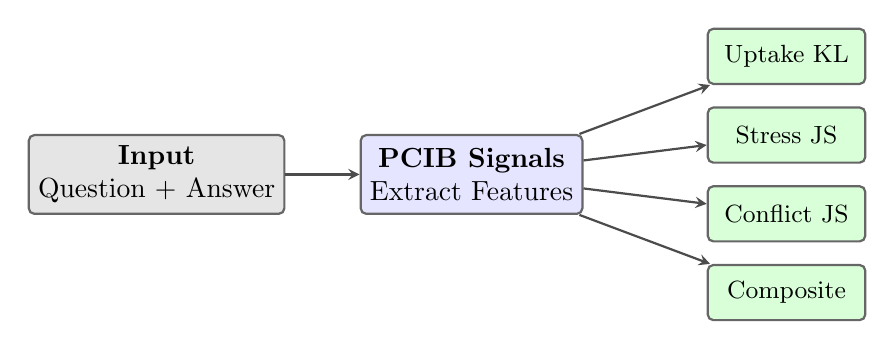
\begin{tikzpicture}[
    box/.style={rectangle, draw=black!60, fill=blue!10, thick, minimum width=2.5cm, minimum height=1cm, align=center, rounded corners=2pt},
    arrow/.style={->, >=stealth, thick, black!70},
    signal/.style={rectangle, draw=black!60, fill=green!15, thick, minimum width=2cm, minimum height=0.7cm, align=center, rounded corners=2pt, font=\small}
]

% Input
\node[box, fill=gray!20] (input) at (0,0) {\textbf{Input}\\Question + Answer};

% PCIB Extraction
\node[box] (pcib) at (4,0) {\textbf{PCIB Signals}\\Extract Features};

% Signals
\node[signal] (uptake) at (8, 1.5) {Uptake KL};
\node[signal] (stress) at (8, 0.5) {Stress JS};
\node[signal] (conflict) at (8, -0.5) {Conflict JS};
\node[signal] (composite) at (8, -1.5) {Composite};

% Arrows
\draw[arrow] (input) -- (pcib);
\draw[arrow] (pcib) -- (uptake);
\draw[arrow] (pcib) -- (stress);
\draw[arrow] (pcib) -- (conflict);
\draw[arrow] (pcib) -- (composite);

\end{tikzpicture}
\caption{\textbf{PCIB Signal Extraction Pipeline.} The framework takes question-answer pairs and extracts four interpretable signals: Uptake (context utilization via KL divergence), Stress (semantic stability via JS divergence), Conflict (logical consistency), and a weighted Composite score.}
\label{fig:pcib_pipeline}
\end{figure}

% Figure: Feature Engineering Process
\begin{figure}[htbp]
\centering
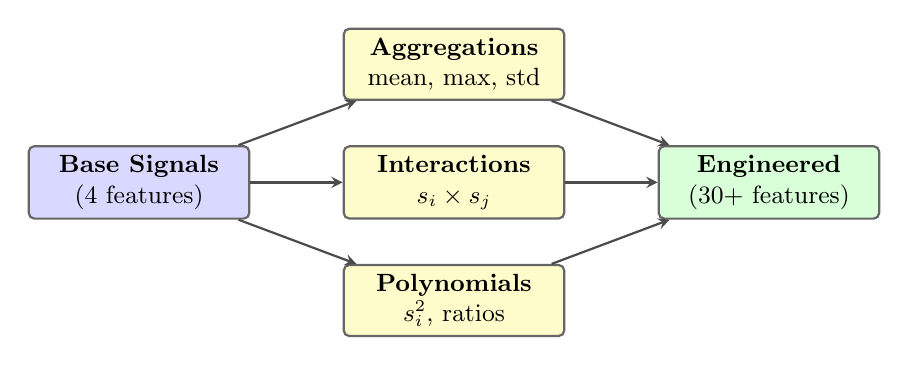
\begin{tikzpicture}[
    box/.style={rectangle, draw=black!60, thick, minimum width=2.8cm, minimum height=0.9cm, align=center, rounded corners=2pt, font=\small},
    arrow/.style={->, >=stealth, thick, black!70}
]

% Base signals
\node[box, fill=blue!15] (base) at (0,0) {\textbf{Base Signals}\\(4 features)};

% Feature engineering steps
\node[box, fill=yellow!20] (agg) at (4,1.5) {\textbf{Aggregations}\\mean, max, std};
\node[box, fill=yellow!20] (inter) at (4,0) {\textbf{Interactions}\\$s_i \times s_j$};
\node[box, fill=yellow!20] (poly) at (4,-1.5) {\textbf{Polynomials}\\$s_i^2$, ratios};

% Engineered features
\node[box, fill=green!15] (eng) at (8,0) {\textbf{Engineered}\\(30+ features)};

% Arrows
\draw[arrow] (base) -- (agg);
\draw[arrow] (base) -- (inter);
\draw[arrow] (base) -- (poly);
\draw[arrow] (agg) -- (eng);
\draw[arrow] (inter) -- (eng);
\draw[arrow] (poly) -- (eng);

\end{tikzpicture}
\caption{\textbf{Feature Engineering Process.} Base PCIB signals are transformed through aggregations (mean, max, std across claims), interactions (pairwise and three-way products), and polynomial terms (squares, ratios) to create 30+ engineered features that capture non-linear patterns.}
\label{fig:feature_engineering}
\end{figure}

% Figure: Stacking Architecture
\begin{figure}[htbp]
\centering
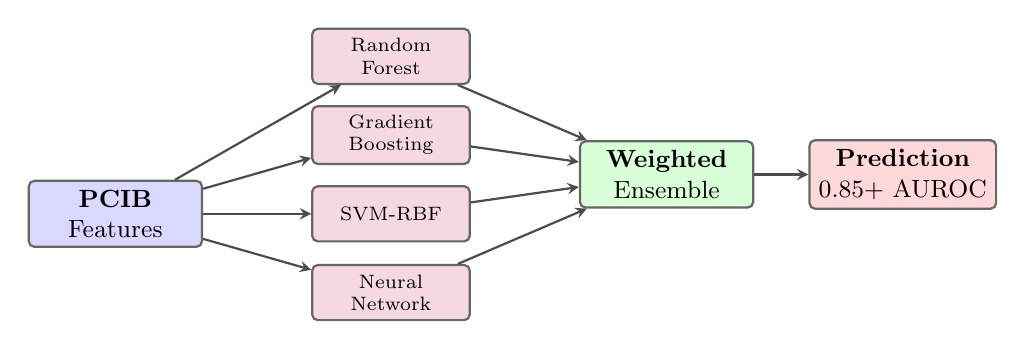
\begin{tikzpicture}[
    box/.style={rectangle, draw=black!60, thick, minimum width=2.2cm, minimum height=0.8cm, align=center, rounded corners=2pt, font=\small},
    model/.style={rectangle, draw=black!60, fill=purple!15, thick, minimum width=2cm, minimum height=0.7cm, align=center, rounded corners=2pt, font=\scriptsize},
    arrow/.style={->, >=stealth, thick, black!70}
]

% Input features
\node[box, fill=blue!15] (features) at (0,0) {\textbf{PCIB}\\Features};

% Models
\node[model] (rf) at (3.5, 2) {Random\\Forest};
\node[model] (gb) at (3.5, 1) {Gradient\\Boosting};
\node[model] (svm) at (3.5, 0) {SVM-RBF};
\node[model] (nn) at (3.5, -1) {Neural\\Network};

% Ensemble
\node[box, fill=green!15] (ensemble) at (7, 0.5) {\textbf{Weighted}\\Ensemble};

% Output
\node[box, fill=red!15] (output) at (10, 0.5) {\textbf{Prediction}\\0.85+ AUROC};

% Arrows
\draw[arrow] (features) -- (rf);
\draw[arrow] (features) -- (gb);
\draw[arrow] (features) -- (svm);
\draw[arrow] (features) -- (nn);
\draw[arrow] (rf) -- (ensemble);
\draw[arrow] (gb) -- (ensemble);
\draw[arrow] (svm) -- (ensemble);
\draw[arrow] (nn) -- (ensemble);
\draw[arrow] (ensemble) -- (output);

\end{tikzpicture}
\caption{\textbf{Stacking Architecture.} Engineered PCIB features are fed to multiple supervised learning models. An optimized weighted ensemble combines predictions to achieve 0.85+ AUROC, balancing the strengths of tree-based, kernel-based, and neural approaches.}
\label{fig:stacking_architecture}
\end{figure}

% Figure: Dual-Mode Framework
\begin{figure}[htbp]
\centering
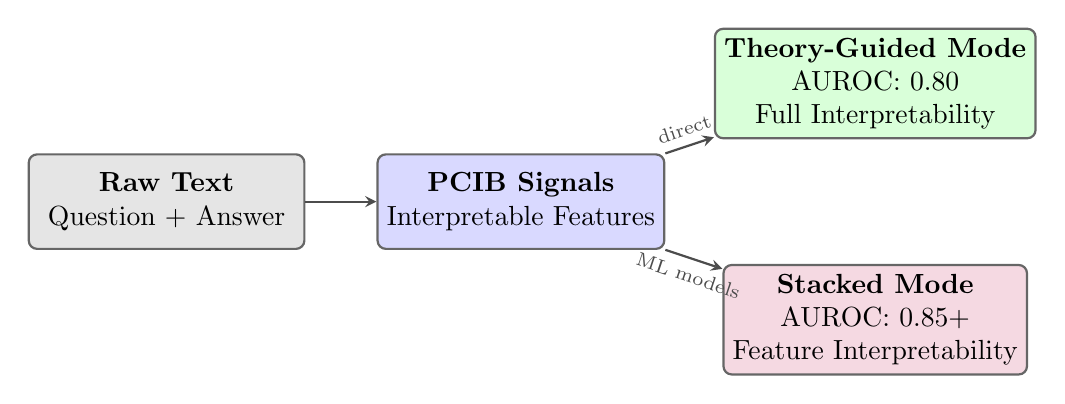
\begin{tikzpicture}[
    box/.style={rectangle, draw=black!60, thick, minimum width=3.5cm, minimum height=1.2cm, align=center, rounded corners=3pt},
    arrow/.style={->, >=stealth, thick, black!70}
]

% Input
\node[box, fill=gray!20] (input) at (0,0) {\textbf{Raw Text}\\Question + Answer};

% PCIB Extraction
\node[box, fill=blue!15] (pcib) at (4.5,0) {\textbf{PCIB Signals}\\Interpretable Features};

% Two modes
\node[box, fill=green!15] (theory) at (9, 1.5) {\textbf{Theory-Guided Mode}\\AUROC: 0.80\\Full Interpretability};
\node[box, fill=purple!15] (stacked) at (9, -1.5) {\textbf{Stacked Mode}\\AUROC: 0.85+\\Feature Interpretability};

% Arrows
\draw[arrow] (input) -- (pcib);
\draw[arrow] (pcib) -- (theory) node[midway, above, sloped, font=\scriptsize] {direct};
\draw[arrow] (pcib) -- (stacked) node[midway, below, sloped, font=\scriptsize] {ML models};

\end{tikzpicture}
\caption{\textbf{Dual-Mode Framework.} PCIB offers flexible deployment: Theory-Guided mode (AUROC 0.80) for full interpretability in high-stakes domains, or Stacked mode (AUROC 0.85+) for competitive performance while maintaining feature-level interpretability. Users choose based on domain requirements.}
\label{fig:dual_mode}
\end{figure}
